\documentclass{article}
\usepackage[utf8]{inputenc}
\usepackage{amsmath}
\usepackage{amssymb}
\usepackage{wasysym}
\usepackage{amsfonts} 
\usepackage{graphicx}
\usepackage{hyperref}
\usepackage[mathscr]{euscript}
\usepackage{geometry}
\usepackage{subfig}
\usepackage{float}
\geometry{left=2.5cm,right=2.5cm,top=2.5cm,bottom=2.5cm}

\newcommand{\resistor}[1]{$\text{#1} \Omega \text{ Resistor}$}

\title{Soldering Guide \\
\large CHARM}
\author{Martin Michalski}

\begin{document}

\maketitle

\section{USB-C Port}

\subsection{Materials}
Begin by retrieving the components in \autoref{tbl:usbc-materials}.

\begin{table}[H]
    \begin{center}
        \begin{tabular}{ c|c|c|c } 
            \textbf{Part No.} & \textbf{Description} & \textbf{Silkscreen No(s).} & \textbf{Quantity} \\ 
            \hline
            USB4140-GF-0070-C & USB-C Port & J1 & 1 \\ 
            \hline
            SF-1206F250-2 & 2.5A Fuse  & F1 & 1 \\ 
            \hline
            RT0603DRE075K1L & \resistor{5.1k} & R3,R6 & 2   \\ 
            \hline
            RT0603FRE131KL & \resistor{1k} & R5 & 1\\ 
            \hline
            150080RS75000 & USB LED & D1 & 1\\ 
        \end{tabular}
    \end{center}
    \caption{Required Components for USB-C Subsystem}
    \label{tbl:usbc-materials}
\end{table}

\subsection{Layout}

Reference \autoref{fig:usbc-layout} to properly place the components.

\begin{figure}[H]
    \centering
        \subfloat[\centering Soldered Example]{{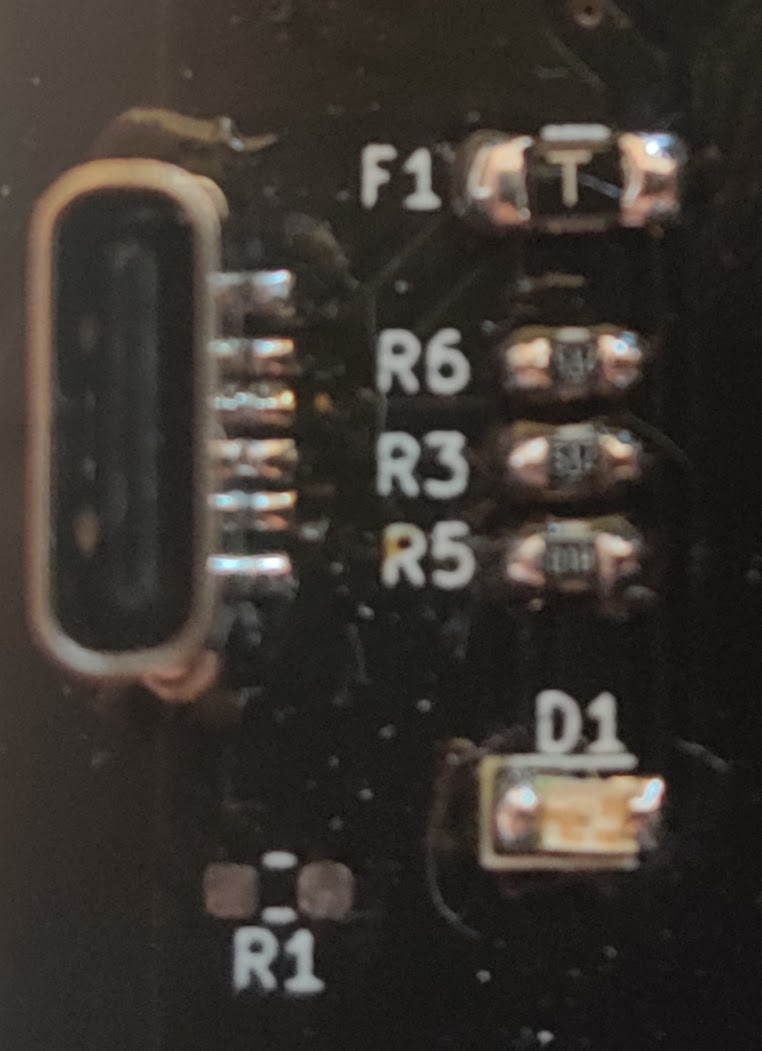
\includegraphics[height=6cm]{./images/usb_real.jpg} }}%
        \qquad
        \subfloat[\centering PCB Layout]{{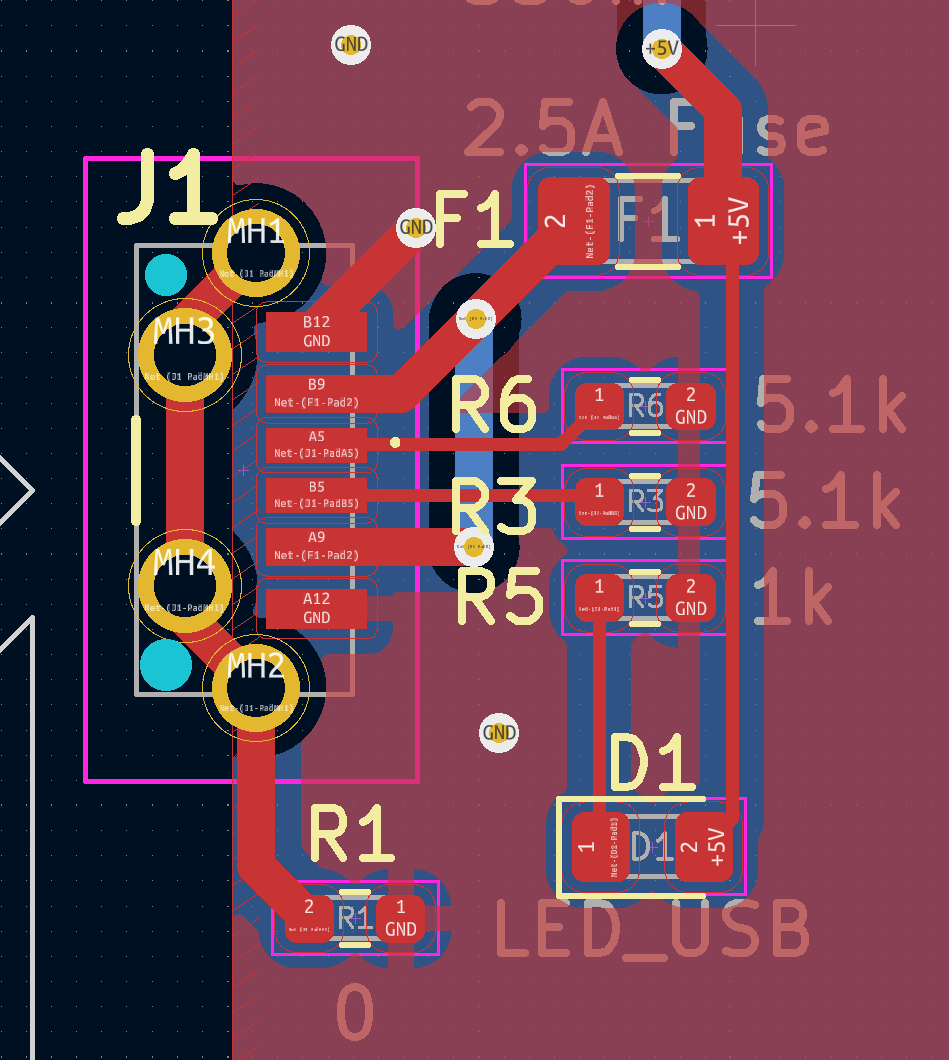
\includegraphics[height=6cm]{./images/usb_pcb_kicad.png} }}%
        \caption{USB-C Subsystem Layout Reference}%
    \label{fig:usbc-layout}%
\end{figure}

\noindent \textbf{Polarity Notes}\\
\noindent \textit{Pay special attention to the orientation of the following components.}
\begin{itemize}
  \item D1: USB LED (Arrow towards H1/H3 side of board)
\end{itemize}

\subsection{Soldering}

Solder the components. \\

\noindent \textbf{Recommended Order}

\begin{enumerate}
  \item F1: 2.5A Fuse
  \item R6: \resistor{5.1k}
  \item R3: \resistor{5.1k}
  \item R5: \resistor{1k}
  \item D1: USB LED
  \item J1: USB-C Port
\end{enumerate}

\noindent \textit{Do not solder R1.}

\subsection{Quality Assurance}

TREVOR TODO

\section{Boost Converter}

\subsection{Materials}
Begin by retrieving the components in \autoref{tbl:boost-materials}.

\begin{figure}[H]
    \begin{center}
        \begin{tabular}{ c|c|c|c } 
            \textbf{Part No.} & \textbf{Description} & \textbf{Silkscreen No(s).} & \textbf{Quantity} \\ 
            \hline
            LM2585S-12/NOPB & Boost Converter IC & IC3 & 1 \\ 
            \hline
            UUD1C221MCL1GS & 220uF Capacitor & C7 & 1 \\ 
            \hline
            16SVPF1000M & 1mF Capacitor & C9 & 1 \\ 
            \hline
            ECPU1C334MA5 & 330nF Capacitor & C2 & 1 \\ 
            \hline
            MSS1210-683MED & 68uH Inductor & L2 & 1 \\ 
            \hline
            RC0603FR-072K94L & \resistor{2.94k} & R7 & 1 \\
            \hline
            SS24FL & Schottky Diode & D4 & 1 
        \end{tabular}
    \end{center}
    \caption{Required Components for Boost Converter Subsystem}
    \label{tbl:boost-materials}
\end{figure}

\subsection{Layout}

Reference \autoref{fig:boost-layout} to properly place the components.

\begin{figure}[H]
    \centering
        \subfloat[\centering Soldered Example]{{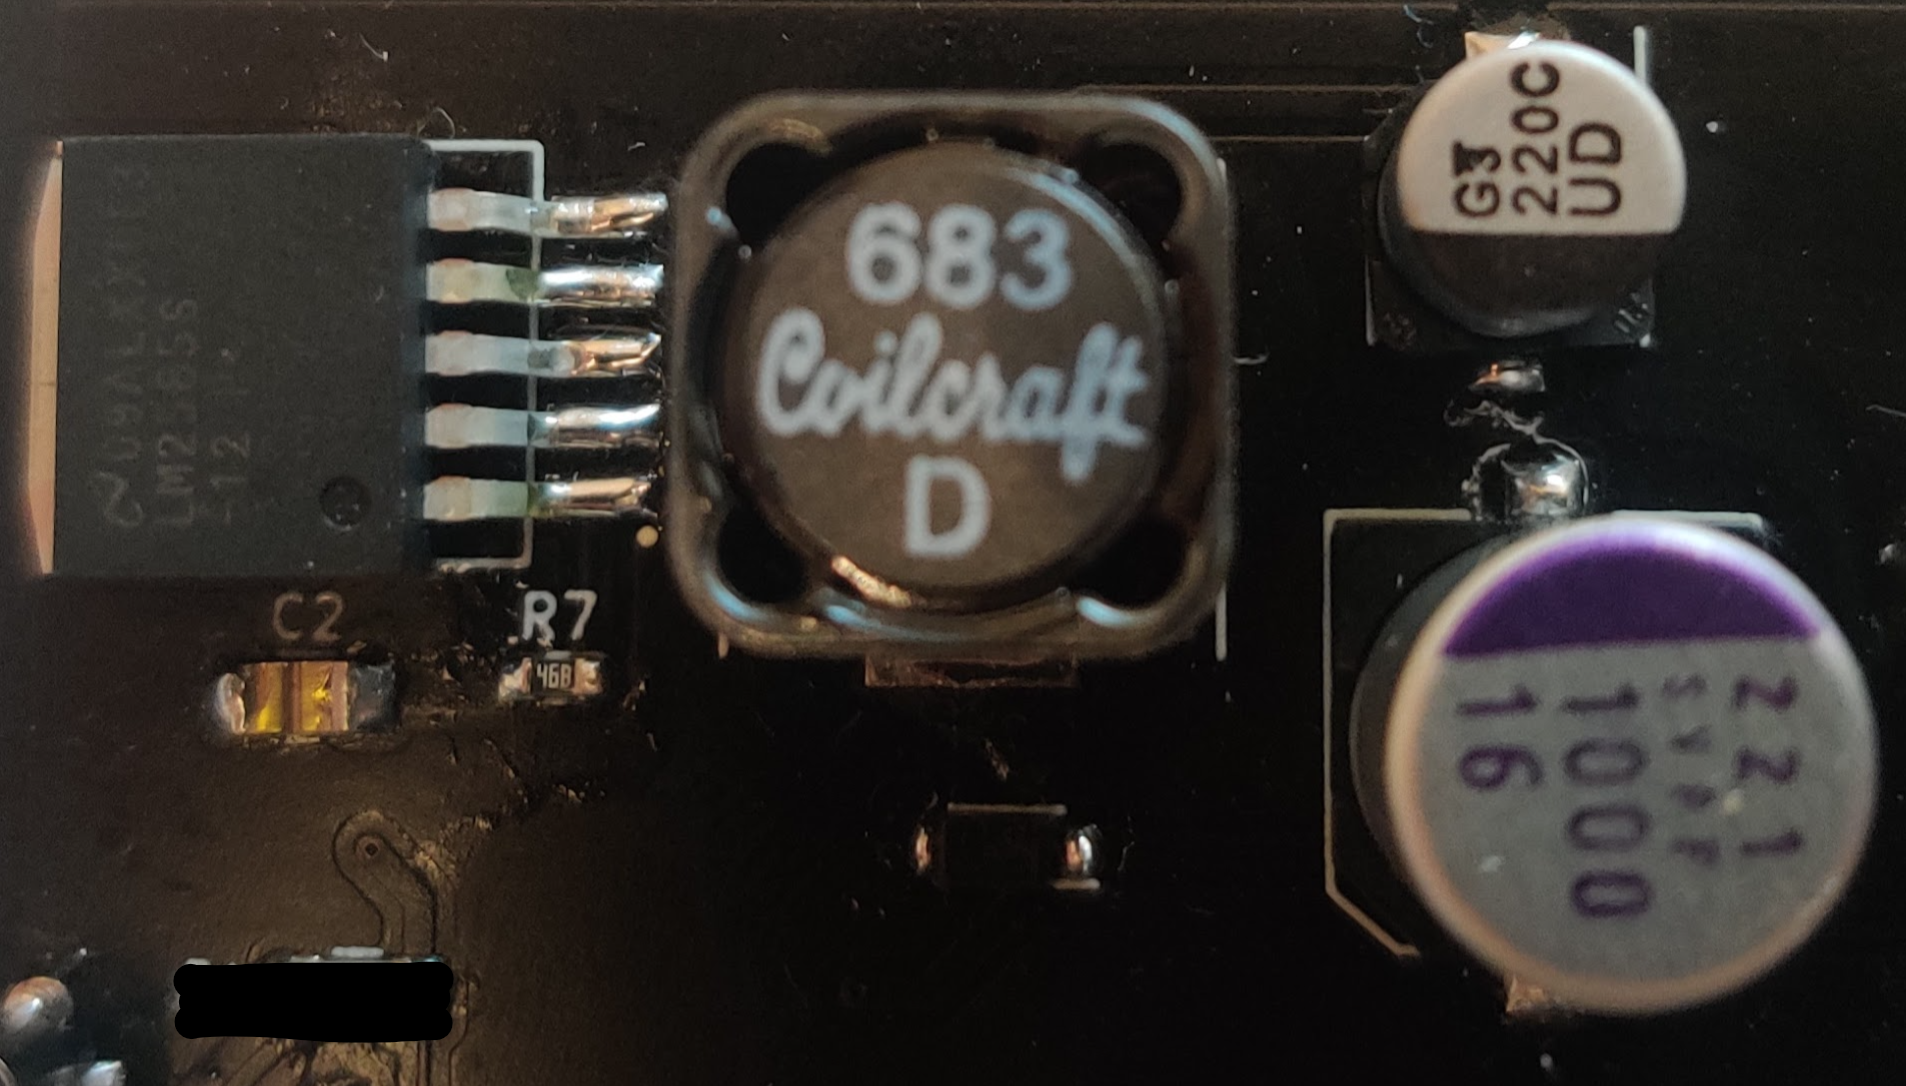
\includegraphics[height=4.5cm]{./images/boost_real.png} }}%
        \qquad
        \subfloat[\centering PCB Layout]{{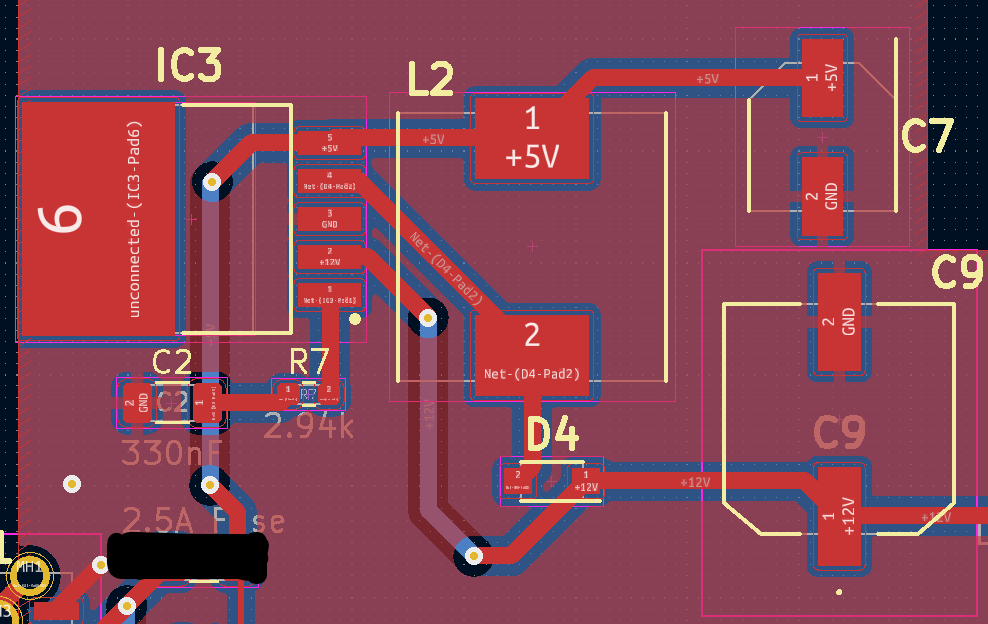
\includegraphics[height=4.5cm]{./images/boost_pcb_kicad.png} }}%
        \caption{Boost Converter Subsystem Layout Reference}%
    \label{fig:boost-layout}%
\end{figure}

\noindent \textbf{Polarity Notes}\\
\noindent \textit{Pay special attention to the orientation of the following components.}
\begin{itemize}
  \item C9: 1mF Capacitor (Reference \autoref{fig:boost-layout}.a)
  \item C7: 220uF Capacitor (Reference \autoref{fig:boost-layout}.a)
  \item C2: TODO TREVOR
  \item D4: TODO TREVOR
\end{itemize}

\subsection{Soldering}

Solder the components. \\

\noindent \textbf{Recommended Order}

\begin{enumerate}
  \item IC3: Boost Converter IC 
  \item C2: 330nF Capacitor
  \item R7: \resistor{2.94k}
  \item D4: Schottky Diode 
  \item L2: 68uH Inductor
  \item C7: 1mF Capacitor
  \item C9: 220uF Capacitor
\end{enumerate}

\subsection{Quality Assurance}

\section{Battery Charge Controller}

\subsection{Materials}
Begin by retrieving the components in \autoref{tbl:charge-materials}.

\begin{figure}[H]
    \begin{center}
        \begin{tabular}{ c|c|c|c } 
            \textbf{Part No.} & \textbf{Description} & \textbf{Silkscreen No(s).} & \textbf{Quantity} \\ 
            \hline
            MCP73844-840I/MS & Battery Charge IC & IC1 & 1 \\ 
            \hline
            EEE-FN1E100R & 10uF Capacitor & C1, C6 & 2 \\ 
            \hline
            T491A104K035AT & 0.1uF Capacitor & C3 & 1 \\ 
            \hline
            RT0603BRD0750KL & \resistor{50k} & R2 & 1 \\ 
            \hline
            ERJ-6RQFR22V & \resistor{220m} & R4 & 1 \\ 
            \hline
            150080RS75000 & Red LED & D2 &  1 \\ 
            \hline
            IRF7404TRPBF & MOSFET & Q1 & 1 \\ 
            \hline
            MCP73844-840I/MS & Battery Holder & J2 & 1 \\ 
            \hline
            L101011MS02Q & Switch & SW1 & 1 
        \end{tabular}
    \end{center}
    \caption{Required Components for the Battery Charge Controller Subsystem}
    \label{tbl:charge-materials}
\end{figure}

\subsection{Layout}

Reference \autoref{fig:charge-layout} to properly place the components.

\begin{figure}[H]
    \centering
        \subfloat[\centering Soldered Example]{{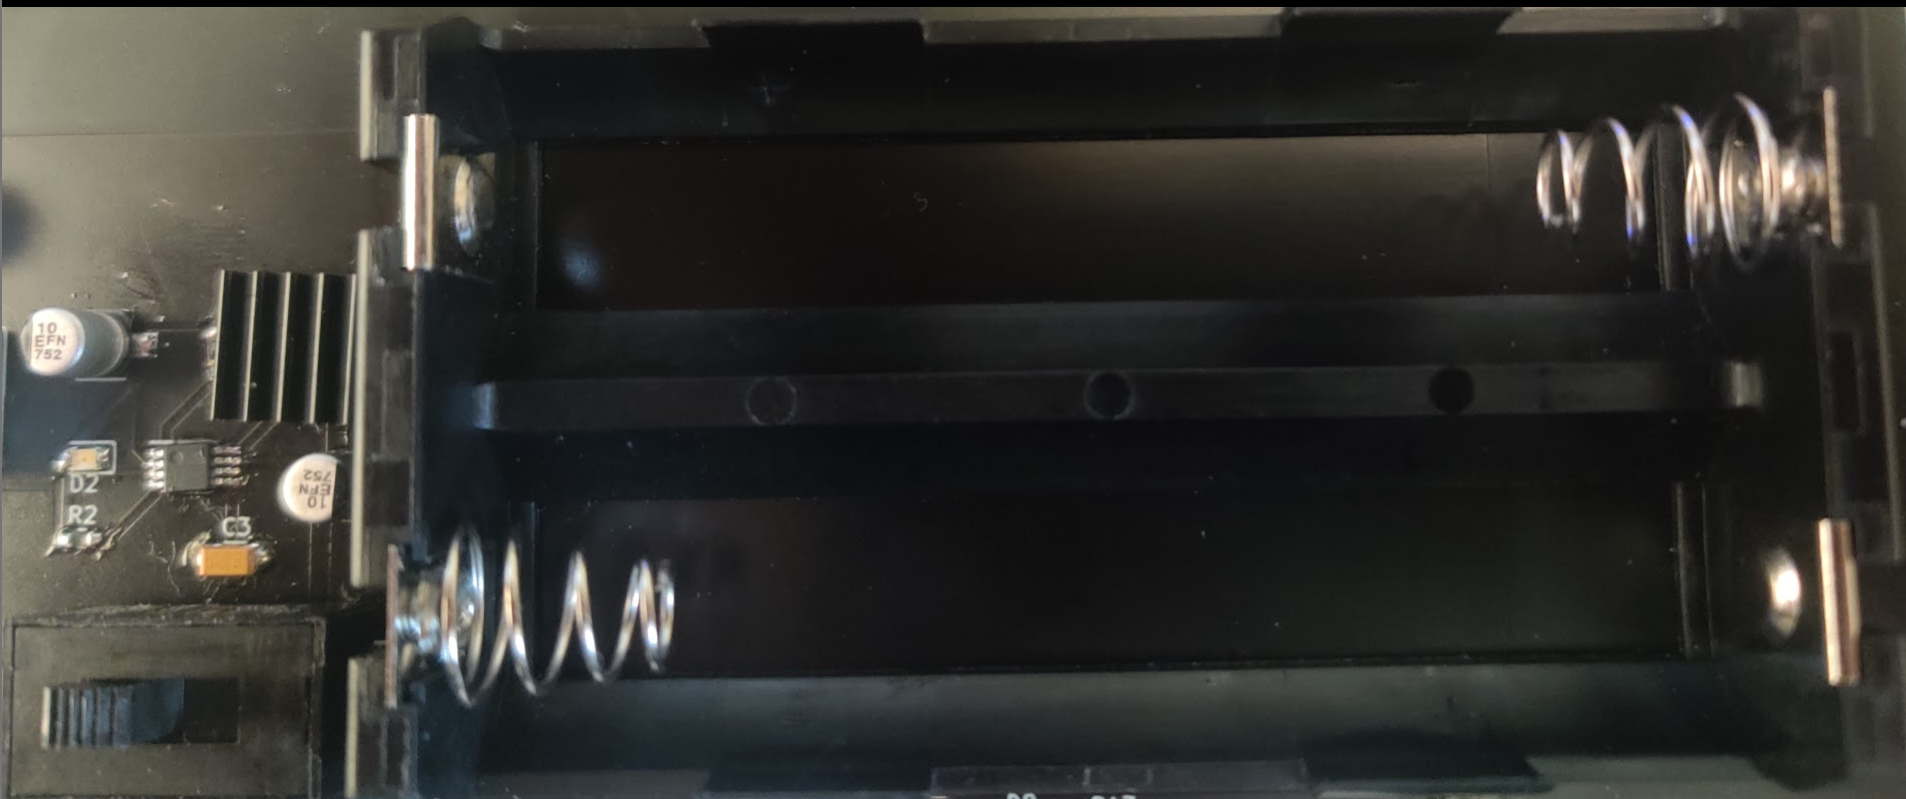
\includegraphics[height=6cm]{./images/charge_real.png} }}%
        \qquad
        \subfloat[\centering PCB Layout]{{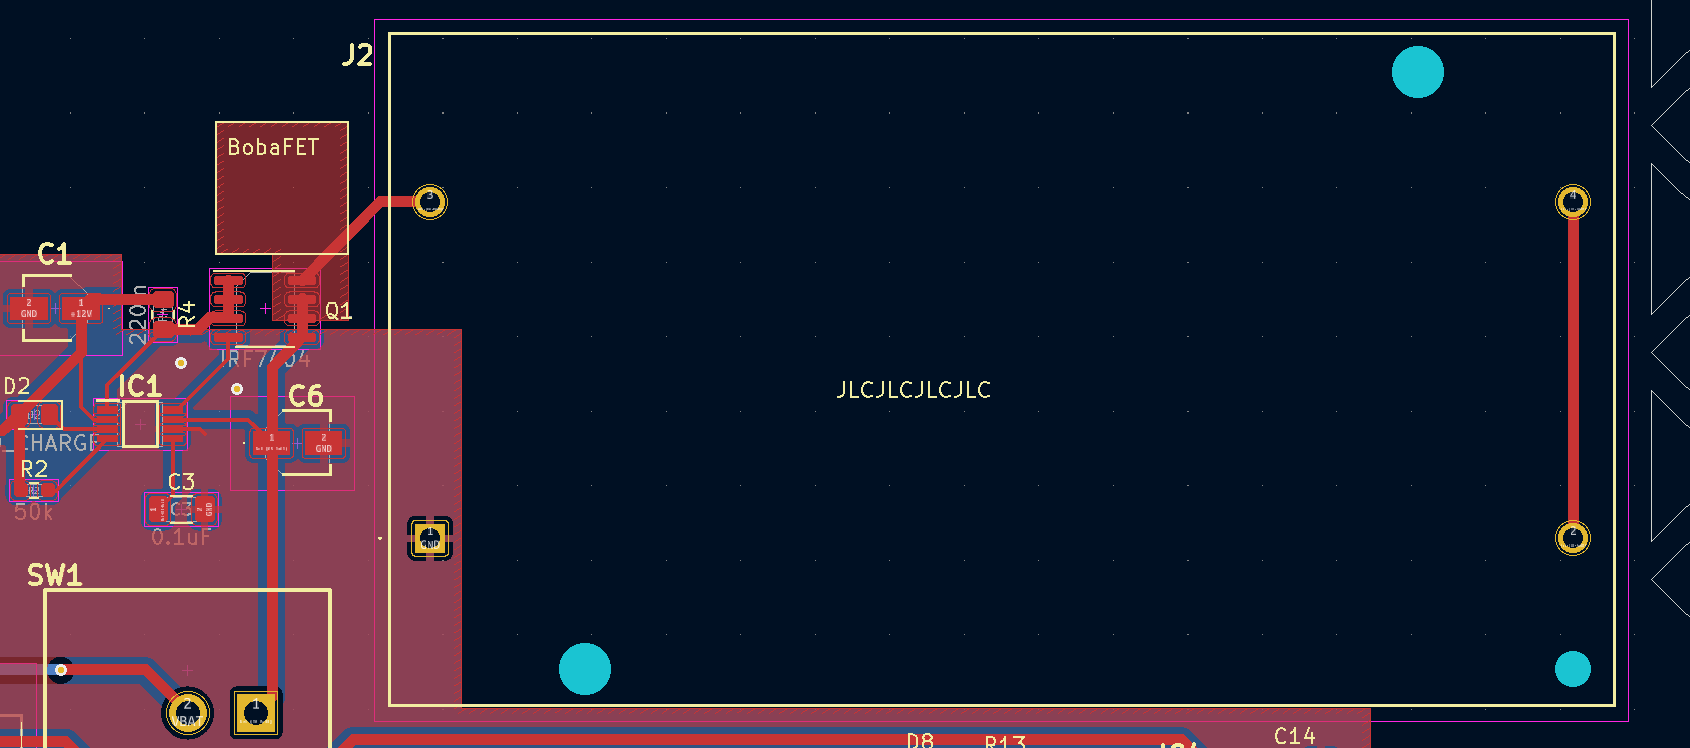
\includegraphics[height=6cm]{./images/charge_pcb_kicad.png} }}%
        \caption{Battery Charge Controller Subsystem Layout Reference}%
    \label{fig:charge-layout}%
\end{figure}

\noindent \textbf{Polarity Notes}\\
\noindent \textit{Pay special attention to the orientation of the following components.}
\begin{itemize}
  \item C1: 10uF Capacitor (Reference \autoref{fig:charge-layout}.a)
  \item C6: 10uF Capacitor (Reference \autoref{fig:charge-layout}.a)
  \item C3: 0.1uF Capacitor  (Banded, bevelled side towards H1/H3 board side)
  \item D2: Red LED (Arrow towards H2/H4 side of board)
  \item IC1: Battery Charge IC (Dot in top-left corner, towards H1 board corner)
  \item Q1: TODO TREVOR
\end{itemize}

\subsection{Soldering}

Solder the components. \\

\noindent \textbf{Recommended Order}

\begin{enumerate}
  \item IC1: Battery Charge IC
  \item Q1: MOSFET
  \item R4: \resistor{220m} 
  \item D2: Red LED
  \item R2: \resistor{50k}
  \item C3: 0.1uF Capacitor
  \item C1, C6: 10uF Capacitors 
  \item SW1: Switch
  \item J2: Battery Holder
\end{enumerate}

After soldering, attach heatsink to BobaFET square.

\subsection{Quality Assurance}

TREVOR TODO

\section{Buck Converter}

\subsection{Materials}
Begin by retrieving the components in \autoref{tbl:buck-materials}.

\begin{figure}[H]
    \begin{center}
        \begin{tabular}{ c|c|c|c } 
            \textbf{Part No.} & \textbf{Description} & \textbf{Silkscreen No(s).} & \textbf{Quantity} \\ 
            \hline
            LM2576SX-3.3/NOPB & Buck Converter IC & IC2 & 1 \\ 
            \hline
            RT0603FRE131KL & \resistor{1k} & R8 & 1 \\ 
            \hline
            16SVPC100M & 100uF Capacitor & C8 & 1 \\ 
            \hline
            UUD1C221MCL1GS & 220uF Capacitor & C4, C5 & 2 \\ 
            \hline
            B520C-13-F & Schottky Diode & D3 & 1 \\ 
            \hline
            150080RS75000 & Red LED & D5 & 1 \\ 
            \hline
            74437429203101 & 100uH Inductor & L1 & 1 \\ 
        \end{tabular}
    \end{center}
    \caption{Required Components for Buck Converter Subsystem}
    \label{tbl:buck-materials}
\end{figure}

\subsection{Layout}

Reference \autoref{fig:buck-layout} to properly place the components.

\begin{figure}[H]
    \centering
        \subfloat[\centering Soldered Example]{{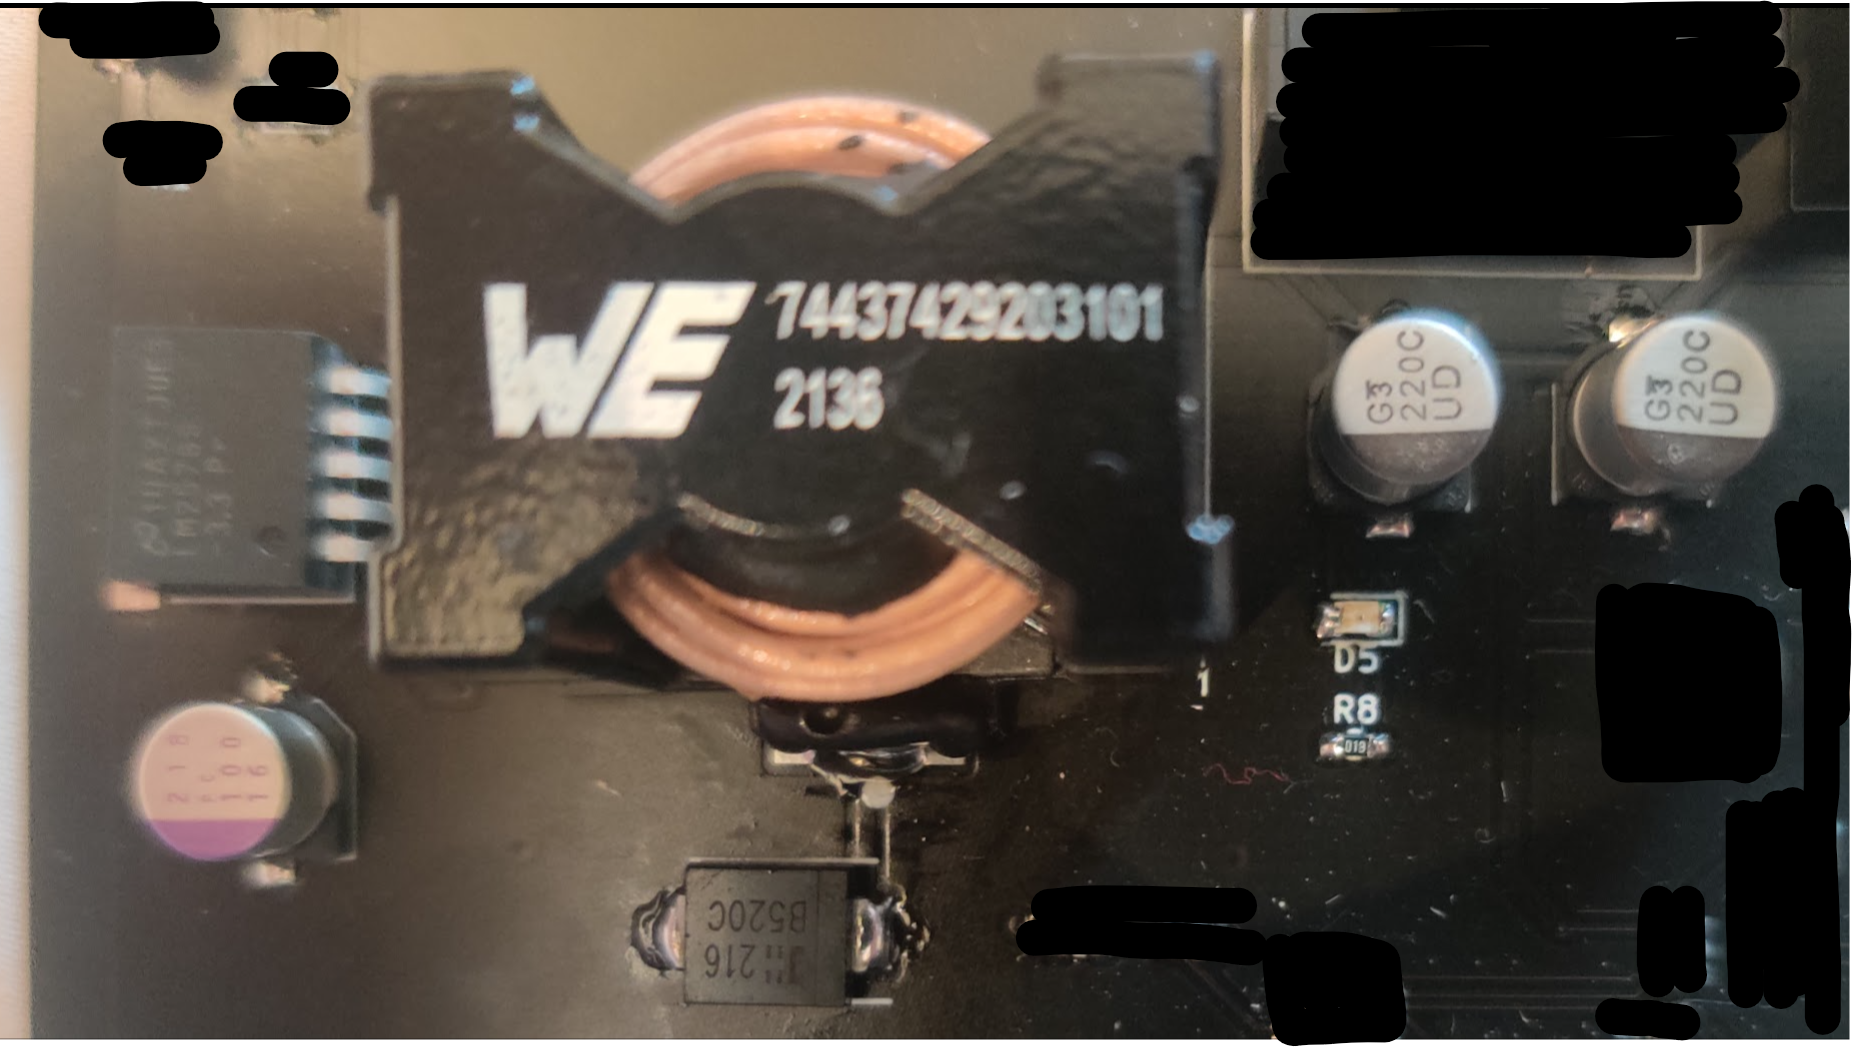
\includegraphics[height=6cm]{./images/buck_real.png} }}%
        \qquad
        \subfloat[\centering PCB Layout]{{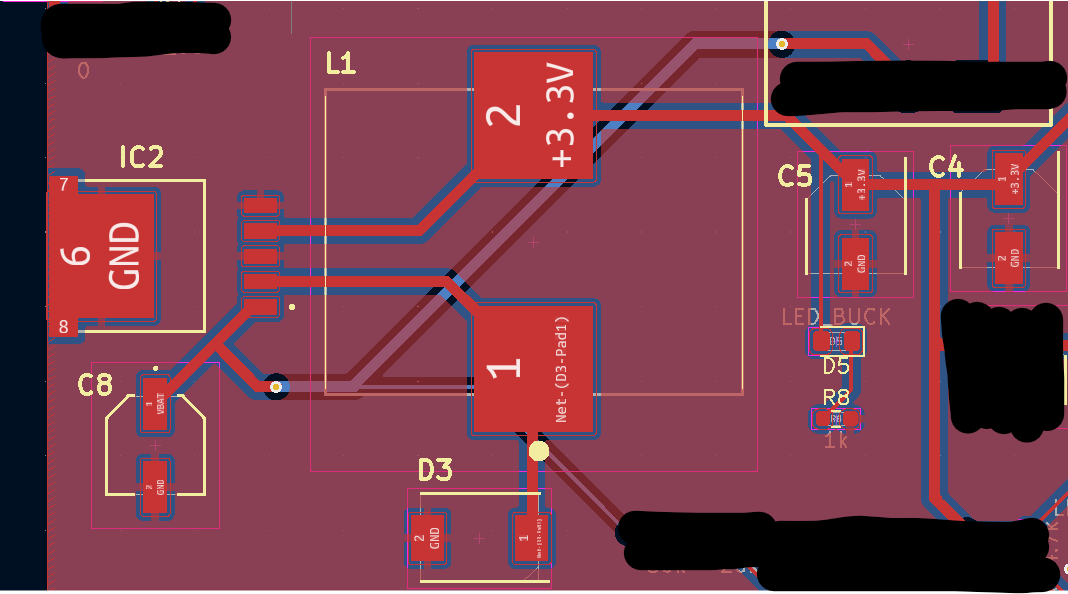
\includegraphics[height=6cm]{./images/buck_pcb_kicad.png} }}%
        \caption{Buck Converter Subsystem Layout Reference}%
    \label{fig:buck-layout}%
\end{figure}

\noindent \textbf{Polarity Notes}\\
\noindent \textit{Pay special attention to the orientation of the following components.}
\begin{itemize}
  \item D3: Schottky Diode (Ensure band is on H2/H4 side of board)
  \item D5: Red LED (Arrow towards H2/H4 side of board) 
  \item C4, C5: 220uF Capacitor (Reference \autoref{fig:buck-layout}.a) 
  \item C8: 100uF Capacitor (Reference \autoref{fig:buck-layout}.a)
\end{itemize}

\subsection{Soldering}

Solder the components. \\

\noindent \textbf{Recommended Order}

\begin{enumerate}
  \item R8: \resistor{1k}
  \item D5: Red LED
  \item D3: Schottky Diode
  \item C4, C5: 220uF Capacitors
  \item C8: 100uF Capacitor
  \item IC2: Buck Converter IC
  \item L1: 100uH Inductor
\end{enumerate}

\subsection{Quality Assurance}

TREVOR TODO

\section{Omega 2S+}

\subsection{Materials}
Begin by retrieving the components in \autoref{tbl:omega-materials}.

\begin{figure}[H]
    \begin{center}
        \begin{tabular}{ c|c|c|c } 
            \textbf{Part No.} & \textbf{Description} & \textbf{Silkscreen No(s).} & \textbf{Quantity} \\ 
            \hline
            OM-O2SP & Omega2S+ & U2 & 1 \\ 
            RT0603BRE0750RL & \resistor{50} & R11 & 1 \\ 
            RT0603FRE131KL & \resistor{1k} & R12 & 1 \\ 
            RT0603BRD0750KL & \resistor{50k} & R21 & 1 \\ 
            150080VS75000 & Green LED & D7 & 1 \\ 
            1N5819 & Schottky Diode & D6 & 1 \\ 
            EEE-FN1E100R & 10uF Capacitor & C12 & 1 \\ 
            T491A104K035AT & 0.1uF Capacitor & C13 & 1 \\ 
        \end{tabular}
    \end{center}
    \caption{Required Components for Omega2S+ Subsystem}
    \label{tbl:omega-materials}
\end{figure}

\subsection{Layout}

Reference \autoref{fig:omega-layout} to properly place the components.

\begin{figure}[H]
    \centering
        \subfloat[\centering Soldered Example]{{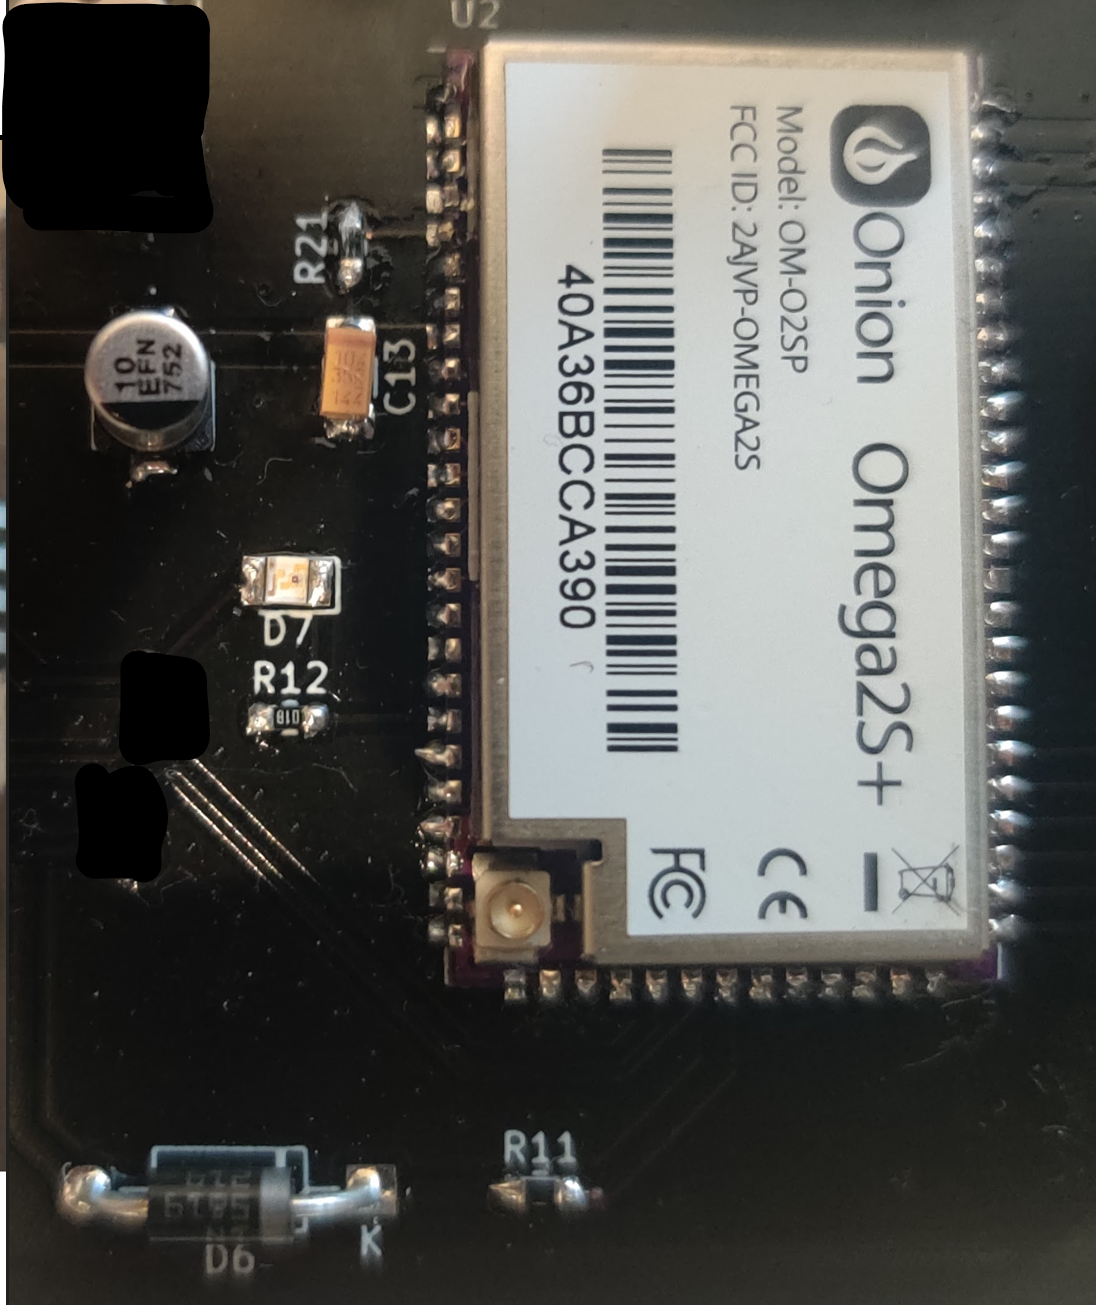
\includegraphics[height=6cm]{./images/omega_real.png} }}%
        \qquad
        \subfloat[\centering PCB Layout]{{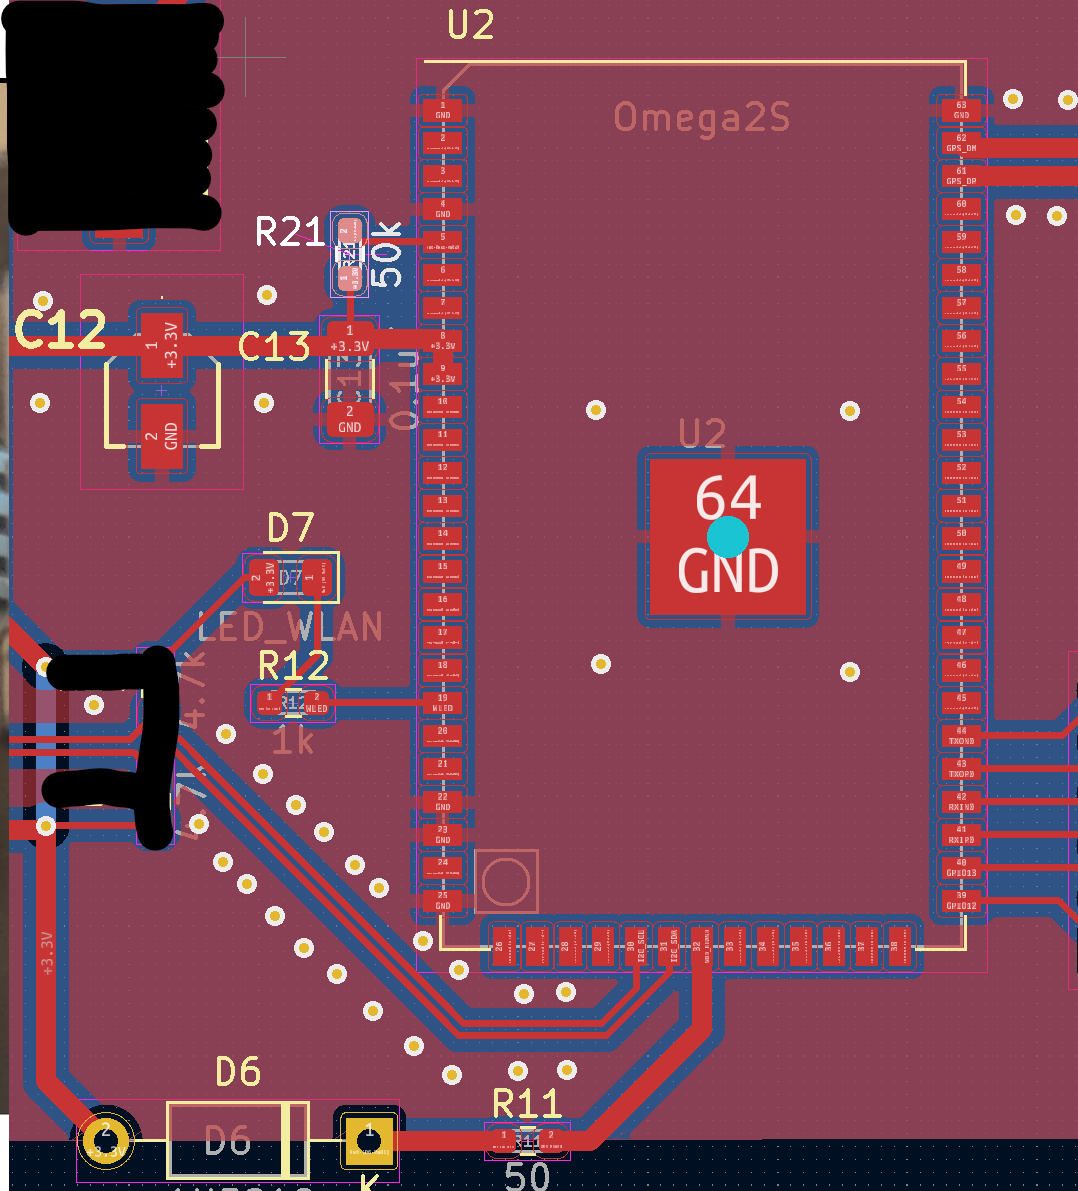
\includegraphics[height=6cm]{./images/omega_pcb_kicad.png} }}%
        \caption{Omega2S+ Subsystem Layout Reference}%
    \label{fig:omega-layout}%
\end{figure}

\noindent \textbf{Polarity Notes}\\
\noindent \textit{Pay special attention to the orientation of the following components.}
\begin{itemize}
  \item C12: 10uF Capacitor (Reference \autoref{fig:omega-layout}.a)
  \item C13: 0.1uF Capacitor (Bevel and band towards H1/H2 side of board)
  \item D6: Schottky Diode (Band towards H2/H4 side of board) 
  \item D7: Green LED (Arrow towards H2/H4 side of board)
\end{itemize}

\subsection{Soldering}

Solder the components. \\

\noindent \textbf{Recommended Order}

\begin{enumerate}
  \item R11: \resistor{50}
  \item R12: \resistor{1k} 
  \item R21: \resistor{50k}
  \item D7: Green LED
  \item D6: Schottky Diode
  \item C12: 10uF Capacitor
  \item C13: 0.1uF Capacitor  
  \item U2: Omega2S+
\end{enumerate}

After soldering, attach antenna to U2's U.FL connector.

\subsection{Quality Assurance}
\label{sec:qual-omega}

\begin{enumerate}
  \item Complete assembly of all previous subsystems in the guide.
  \item Insert two batteries into the PCB battery holder, ensuring switch is in the "off" position.
  \item Flip the switch.
  \item The Omega2S+ LED should light up, begin flashing, and then eventually remain solid.
  \item Once the LED remains solid (should be around 1 minute), check the WiFi networks in the lab. There 
        should be a WiFi network with SSID \texttt{Omega-XXXX} where \texttt{XXXX} are the last two bytes
        of the Omega2S+'s MAC address, in hexadecimal notation.
\end{enumerate}

\section{Battery Monitor Subsystem}

\subsection{Materials}
Begin by retrieving the components in \autoref{tbl:batt-mon-materials}.

\begin{figure}[H]
    \begin{center}
        \begin{tabular}{ c|c|c|c } 
            \textbf{Part No.} & \textbf{Description} & \textbf{Silkscreen No(s).} & \textbf{Quantity} \\ 
            \hline
            ADS1113IDGST & ADC & U1 & 1 \\ 
            RT0603BRD0750KL & \resistor{50k} & R9 & 1 \\ 
            RT0603DRE0720KL & \resistor{20k} & R10 & 1 \\ 
            RT0603DRE074K7L & \resistor{4.7k} & R14, R15 & 2 \\ 
            T491A104K035AT & 0.1uF Capacitor & C10 & 1 \\ 
        \end{tabular}
    \end{center}
    \caption{Required Components for Battery Monitor Subsystem}
    \label{tbl:batt-mon-materials}
\end{figure}

\subsection{Layout}

Reference \autoref{fig:batt-mon-layout} to properly place the components.

\begin{figure}[H]
    \centering
        \subfloat[\centering Soldered Example]{{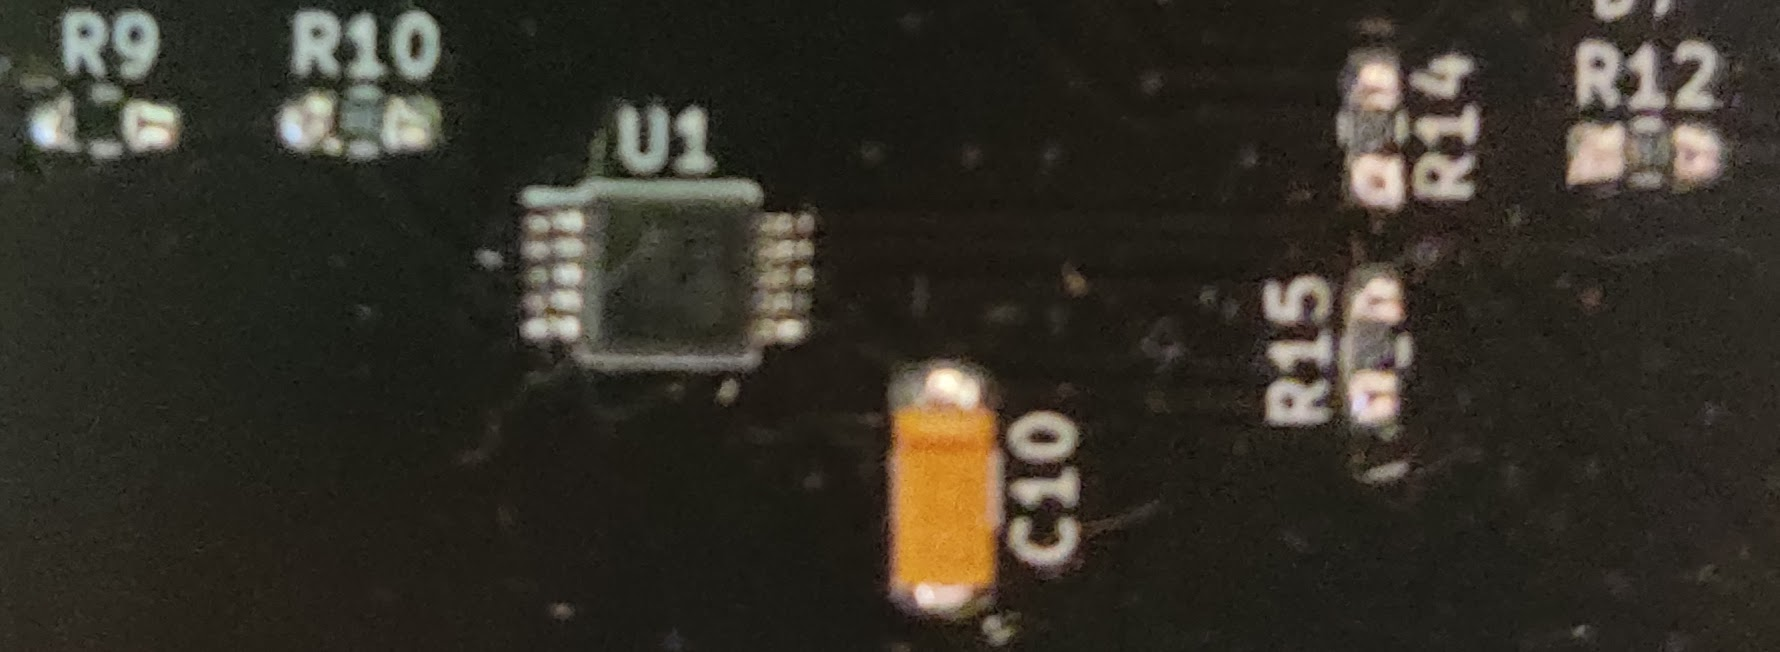
\includegraphics[height=6cm]{./images/batt_mon_real.png} }}%
        \qquad
        \subfloat[\centering PCB Layout]{{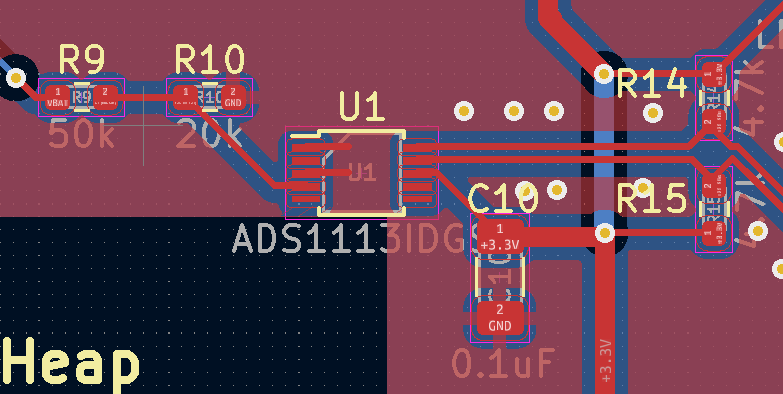
\includegraphics[height=6cm]{./images/batt_mon_pcb_kicad.png} }}%
        \caption{Battery Monitor Subsystem Layout Reference}%
    \label{fig:batt-mon-layout}%
\end{figure}

\noindent \textbf{Polarity Notes}\\
\noindent \textit{Pay special attention to the orientation of the following components}
\begin{itemize}
  \item C10: 0.1uF Capacitor (Bevelled, banded side towards H1/H2 side of the board)
  \item U1: ADC (Dot towards the H1 corner of the board)
\end{itemize}

\subsection{Soldering}

Solder the components. \\

\noindent \textbf{Recommended Order}

\begin{enumerate}
  \item U1: ADC
  \item R9: \resistor{50k}
  \item R10: \resistor{20k}
  \item R14, R15: \resistor{4.7k}
  \item C10: 0.1uF Capacitor
\end{enumerate}

\subsection{Quality Assurance}

\begin{enumerate}
  \item Do the steps in the \hyperref[sec:qual-omega]{Omega2S+ Quality Assurance section}.
  \item Connect to the Omega2S+'s WiFi network.
  \item SSH into the Omega2S+ via the \texttt{ssh root@omega-XXXX.local} command.
  \item Enter the default password when prompted: \texttt{onioneer}.
  \item Download our script for testing the ADC: \texttt{wget TODO}.
  \item Run the script: \texttt{./TODO.sh}.
  \item Measure the voltage of the battery and confirm that it matches that output by the script.
\end{enumerate}

\section{GPS Sensor Subsystem}

\subsection{Materials}
Begin by retrieving the components in \autoref{tbl:gps-materials}.

\begin{figure}[H]
    \begin{center}
        \begin{tabular}{ c|c|c|c } 
            \textbf{Part No.} & \textbf{Description} & \textbf{Silkscreen No(s).} & \textbf{Quantity} \\ 
            \hline
            NEO-M9N-00B & GPS IC & IC4 & 1 \\ 
            C1005X7R1C104K050BC & 100nF Capacitor & C11 & 1 \\ 
            T491A104K035AT & 0.1uF Capacitor & C14 & 1 \\ 
            150080YS75000 & Yellow LED & D8 & 1 \\ 
            AQ3522-01LTG & TVS Diode & D9 & 1 \\ 
            LQW18AN27NG00D & 27nH Inductor & L3 & 1 \\ 
            U.FL-R-SMT(01) & U.FL Connector & J3 & 1 \\ 
            RT0603FRE131KL & \resistor{1k} & R13 & 1 \\ 
            RT1206FRE1310RL & \resistor{10} & R16 & 1 \\ 
        \end{tabular}
    \end{center}
    \caption{Required Components for GPS Sensor Subsystem}
    \label{tbl:gps-materials}
\end{figure}

\subsection{Layout}

Reference \autoref{fig:gps-layout} to properly place the components.

\begin{figure}[H]
    \centering
        \subfloat[\centering Soldered Example]{{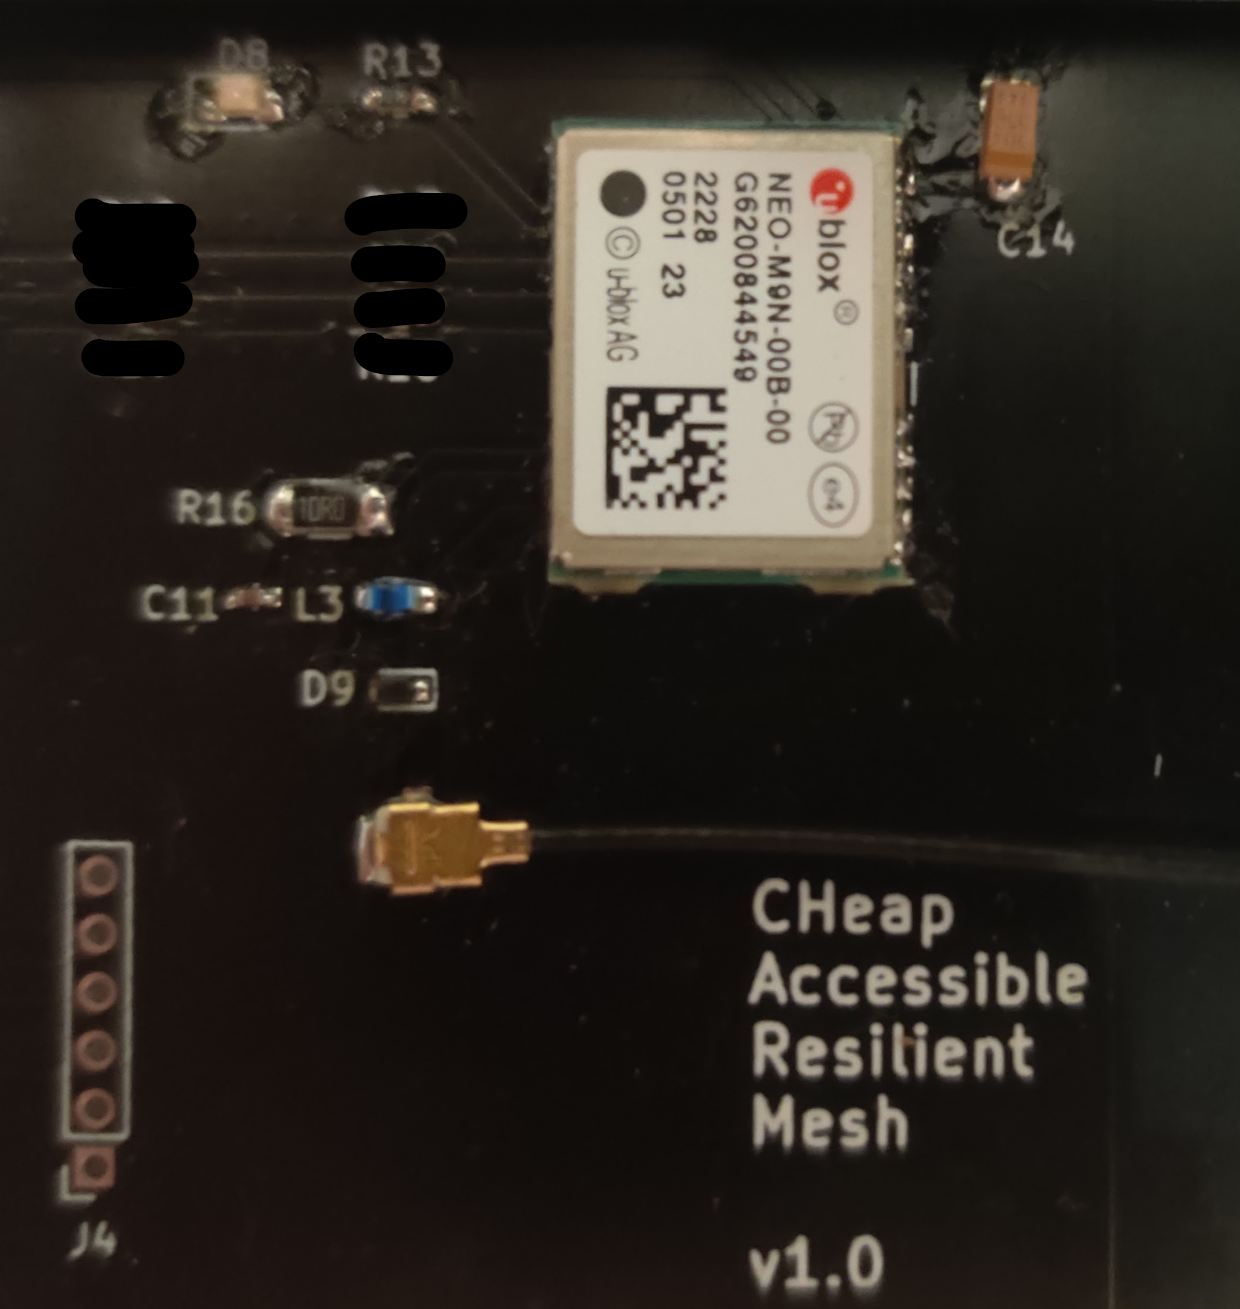
\includegraphics[height=6cm]{./images/gps_real.png} }}%
        \qquad
        \subfloat[\centering PCB Layout]{{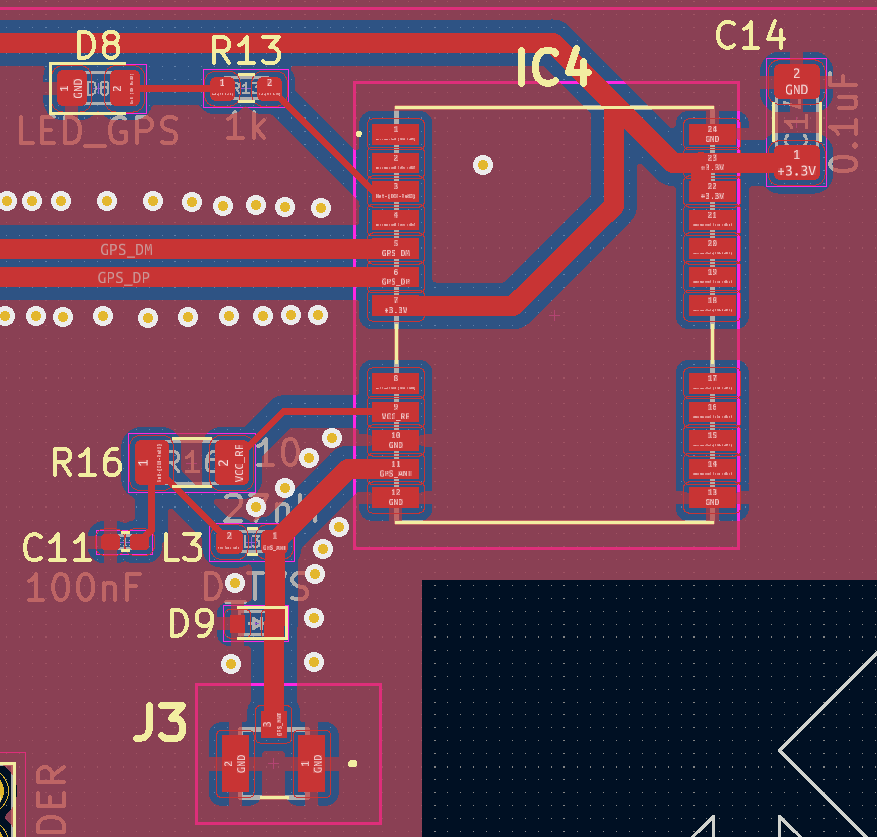
\includegraphics[height=6cm]{./images/gps_pcb_kicad.png} }}%
        \caption{GPS Sensor Subsystem Layout Reference}%
    \label{fig:gps-layout}%
\end{figure}

\noindent \textbf{Polarity Notes}\\
\noindent \textit{Pay special attention to the orientation of the following components}
\begin{itemize}
  \item IC4: GPS IC (Dot towards the H1 corner of the board)
  \item C11: TREVOR TODO
  \item C14: 0.1uF Capacitor (Bevelled, banded edge towards H3/H4 side of the board)
  \item D8: Yellow LED (Arrow towards H1/H3 side of the board)
  \item D9: TREVOR TODO
\end{itemize}

\subsection{Soldering}

Solder the components. \\

\noindent \textbf{Recommended Order}

\begin{enumerate}
  \item IC4: GPS IC
  \item C11: 100nF Capacitor
  \item C14: 0.1uF Capacitor
  \item D8: Yellow LED
  \item D9: TVS Diode
  \item L3: 27nH Inductor
  \item J3: U.FL Connector
  \item R13: \resistor{1k}
  \item R16: \resistor{10}
\end{enumerate}

After soldering, attach GPS antenna to J3.

\subsection{Quality Assurance}

\begin{enumerate}
  \item Do the steps in the \hyperref[sec:qual-omega]{Omega2S+ Quality Assurance section}.
  \item Connect to the Omega2S+'s WiFi network.
  \item SSH into the Omega2S+ via the \texttt{ssh root@omega-XXXX.local} command.
  \item Enter the default password when prompted: \texttt{onioneer}.
  \item Run the following command: \texttt{cat /dev/ttyACM0}.
  \item You should see the output similar to that pictured in \autoref{fig:gps-no-data-output}.
\end{enumerate}

\begin{figure}[H]
    \centering
    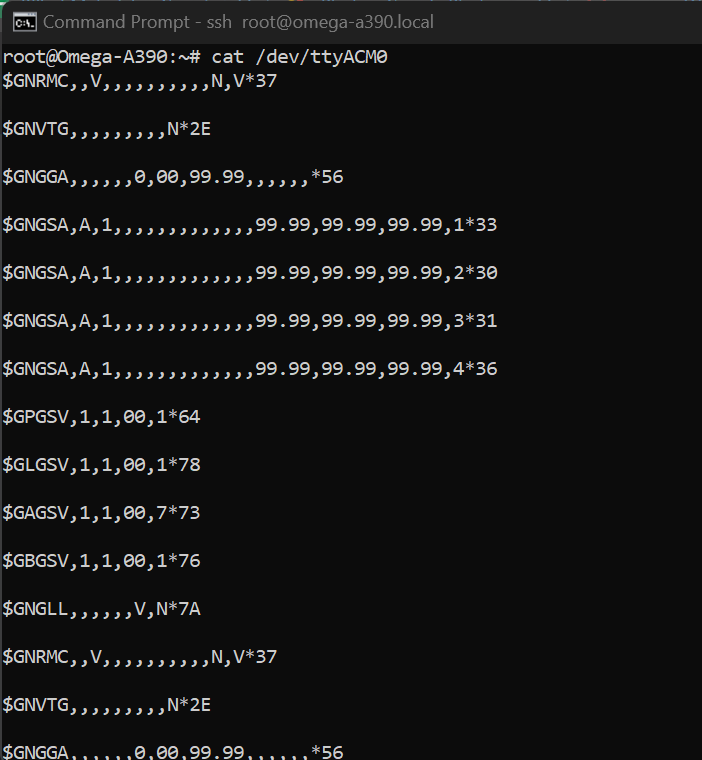
\includegraphics[width=0.5\linewidth]{./images/gps_no_lock_cat_output.png}
    \caption{Expected \texttt{cat /dev/ttyACM0} command output}
    \label{fig:gps-no-data-output}
\end{figure}

\end{document}